\subsubsection{Purpose}
This sub-part of the "Use Car" functionality focuses on the sub-functionalities concerned with the interaction between the user and the on-board application in order to allow the user to turn the engine on.

The system will interact with the user prompting him/her after the car has been unlocked and asking to proceed with the specified authentication method. This process will grant access to the car systems, hence allowing the user to start the ride.

Right after the engine has been ignited, the on-board application will also start charging the user, all while showing him/her the current charges on the screen, along with the sat-nav that is also going to signal nearby charging stations and the boundaries of the Safe Area.

\subsubsection{Scenario 1}
Francis just unlocked the car he reserved using the \emph{PowerEnJoy} service. He sits on the driver's side and closes the door. The screen of the on-board computer is turned on and the system prompts Francis to authenticate. He performs the authentication procedure correctly; the message \emph{"You can now turn the engine on. Once you do so, the system will start charging you based on the duration of the ride."} appears on the screen. Francis turns the engine on and the system shows him his current charges; he then proceeds to drive the car, starting his ride.

\subsubsection{Scenario 2}
Graham mounted on a \emph{PowerEnJoy} vehicle he just reserved and unlocked. When he authenticates after being prompted by the system, he makes an error. The system then shows an error message. Graham then repeats the procedure properly; this time it is correct, and the system allows him to drive the car.

\subsubsection{Use-case}
A detail of the use-case is provided in Table \ref{start_ride_uc}

\subsubsection{Sequence diagram}
A UML sequence diagram is provided to detail the standard behavior of the system upon performance of the authentication method. The diagram is in Figure \ref{start_sd}.

\subsubsection{Functional Requirements}
\begin{enumerate}
\item The system must check that the authentication method is followed properly;
\item The system must start charging the user only after he/she turned the engine on;
\item The system must always notify the user about his/her current charges;
\item The system must mark the car as "in-use" as soon as the engine is ignited;
\end{enumerate}

\begin{figure}[H]
\begin{center}
		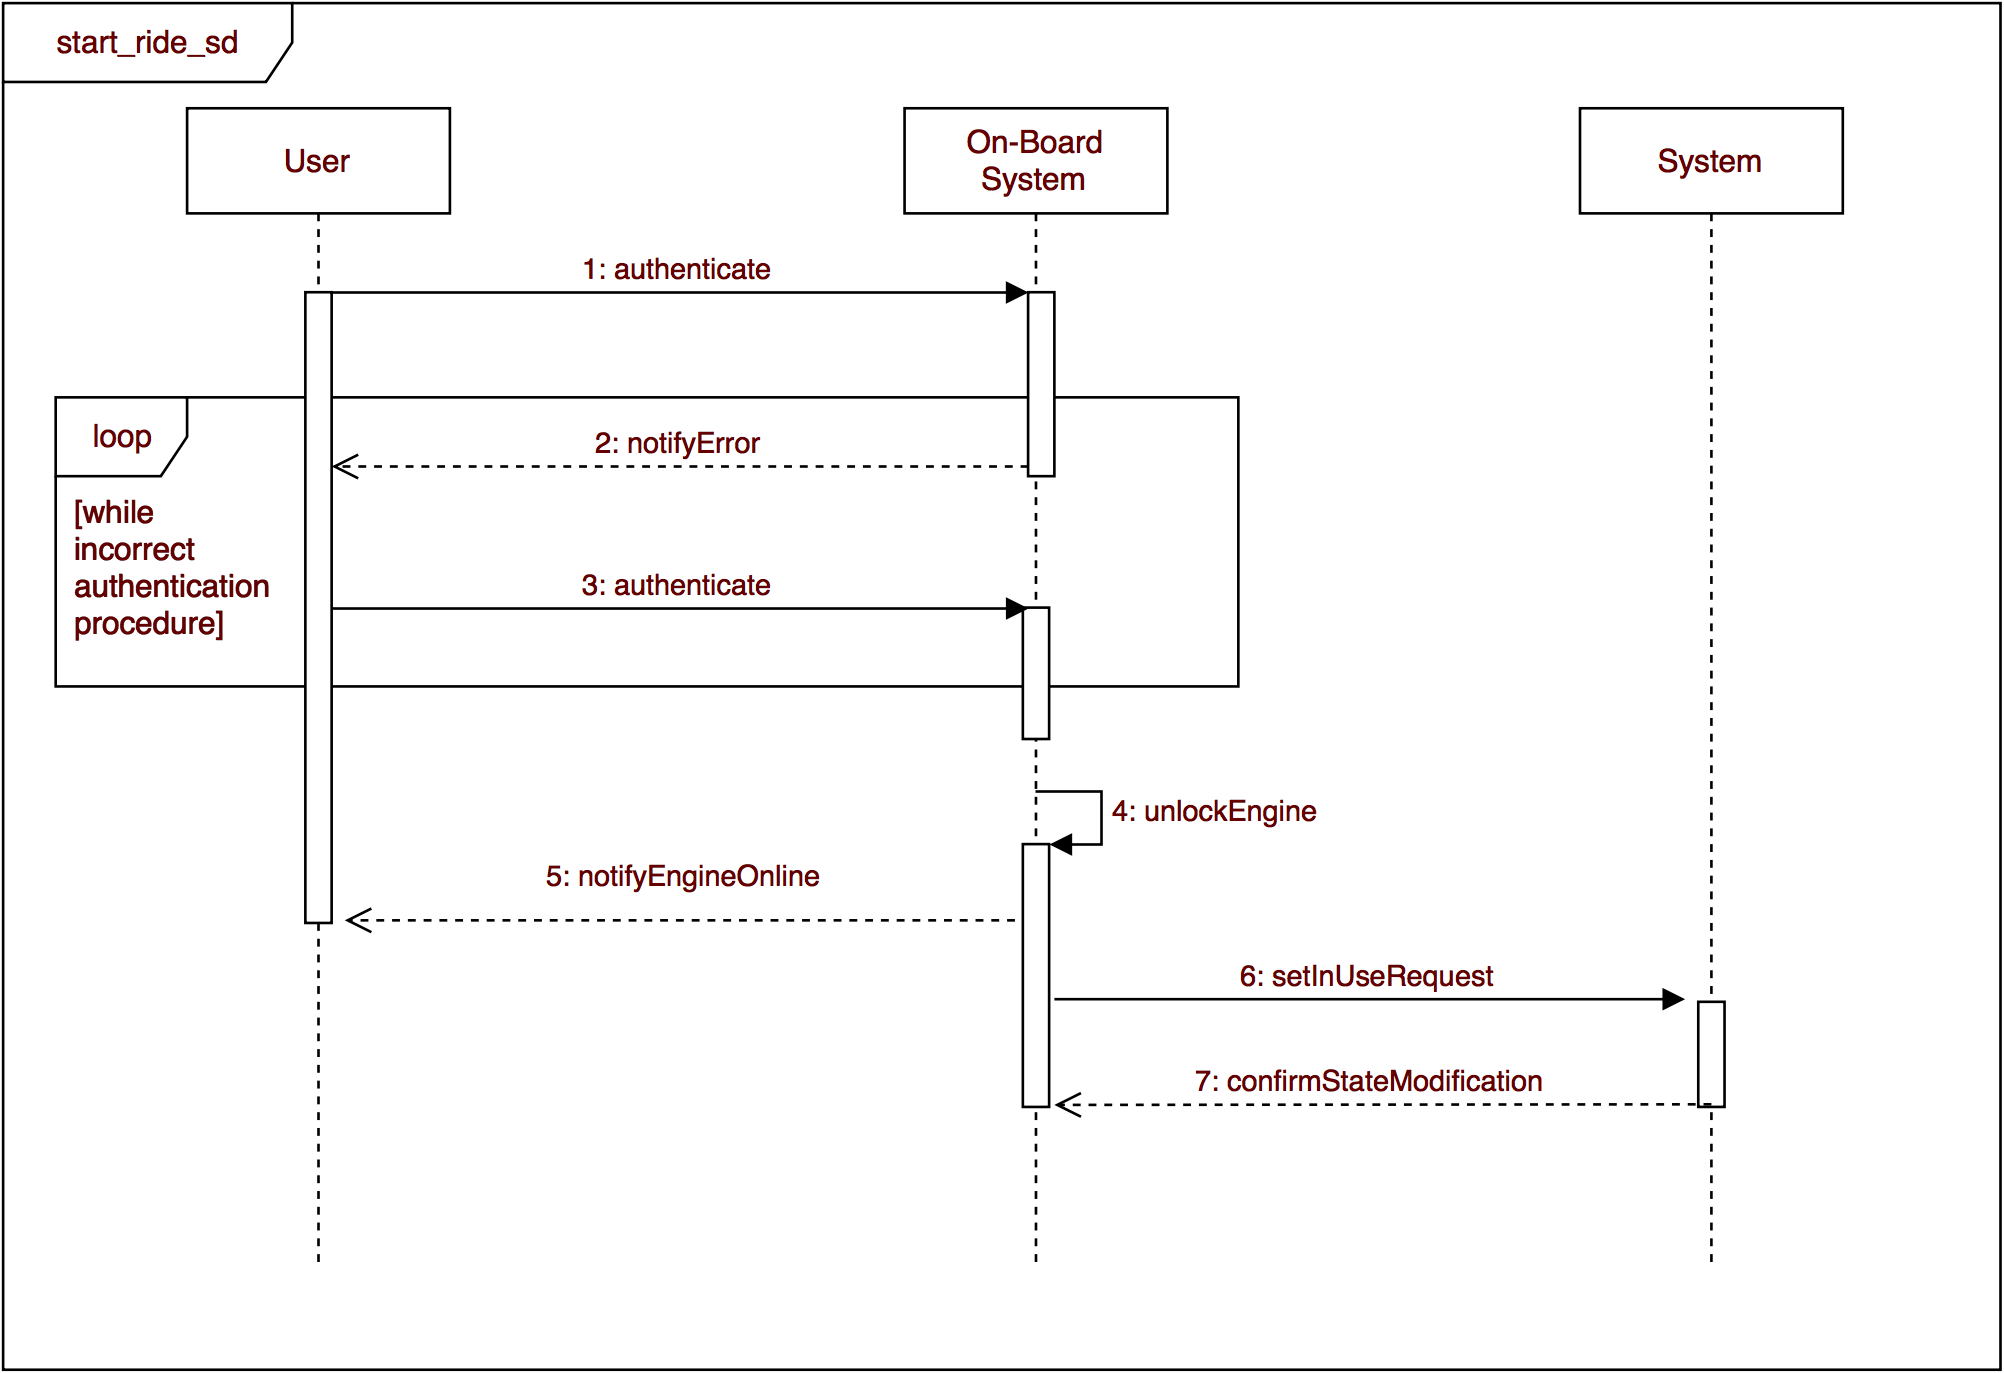
\includegraphics[width=\textwidth]{./specific_requirements/features/diagrams/start_ride_sd.png}
		\caption{Sequence diagram for the process of starting a ride in a standard situation.}
		\label{start_sd}
\end{center}
\end{figure}

\begin{table}[H]
\begin{center}
\begin{tabular}{p{0.3\textwidth} | p{0.7\textwidth}}
\hline
Actor & Logged user\\
\hline
Goal & Goal 7\\
\hline
Input Condition & The user unlocked the car\\
\hline
Event Flow & 
\begin{enumerate}
\item The user performs the authentication procedure interacting with the on-board screen;
\item The system analyzes the procedure correctness;
\item The system opens the possibility for the user to ignite the engine and start his/her ride.
\item The user ignites the engine and starts the ride;
\end{enumerate} \\
\hline
Output Condition & The ride starts, the system starts charging the user. The car status becomes "in-use"\\
\hline
Exception & If the user makes an error while authenticating, the system will notify it and report an error message; in this case, the car still can not be turned on.\\
\hline
\end{tabular}
\end{center}
\caption{Start ride use-case}
\label{start_ride_uc}
\end{table}